\begin{frame}
   \frametitle{Outline}

   \begin{tikzpicture}[font=\small]
      \tikzset{>=latex} % arrow heads
      \draw[step=1,black!15,very thin,opacity=\gridopacity] (0,0) grid (12,8);

      \node[fill=black!5,minimum width=11cm] at (6,7.5) {\strut How to Optimize?};

      \node[fill=blue!10,minimum width=5cm,minimum height=3cm] (lazysp) at (3.25,5.5) {};
      \node[anchor=north] at (lazysp.north) {\strut Lazy Pathfinding};
      \node[draw=black!30,fill=white,inner sep=5pt] at (3.25,5.25) {
         \includegraphics[width=3.8cm]{build/lazysp-icon}};

      \node[fill=blue!10,minimum width=5cm,minimum height=3cm] (ibid) at (8.75,5.5) {};
      \node[anchor=north] at (ibid.north) {\strut Dynamic Pathfinding};
      \node[draw=black!30,inner sep=0pt] at (8.75,5.25) {
         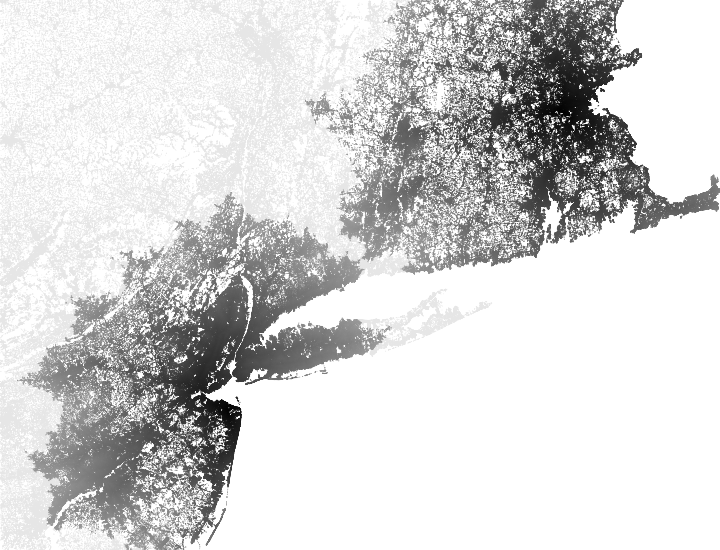
\includegraphics[width=2.9cm]{figs/incbi-road-ne/singleshot/example-bidijkstra.png}};

      \only<2>
      {
         \node[draw,ultra thick,minimum width=5cm,minimum height=3cm] at (ibid) {};
      }

      \node[fill=black!5,minimum width=11cm] at (6,3.5) {\strut What to Optimize?};

      \node[fill=blue!10,minimum width=5cm] at (3,2) {\strut Maximizing Utiliy};

      \node[fill=blue!10,minimum width=5cm] at (9,2) {\strut C-Space Familes};
      
   %Revisit talk outline.
   %LazySP creates a dynamic SP problem underneath.
   %Don't necessarily have good heuristics.

   %Therefore, work on the incremental problem.
   \end{tikzpicture}
\end{frame}

\begin{frame}
   \frametitle{Approaches for Fast Pathfinding}
   \begin{tikzpicture}[font=\small]
      \tikzset{>=latex} % arrow heads
      \draw[step=1,black!15,very thin,opacity=\gridopacity] (0,0) grid (12,8);

      \node[fill=blue!10,minimum width=7cm,minimum height=2.67361cm,align=center] at (4,5.95) {
         Problem:\\
         Dynamic Single-Pair Shortest Path (SPSP)\\
      };

      \begin{scope}[shift={(8.0,4.6)}]
         \node[inner sep=0pt,anchor=south west] {%
            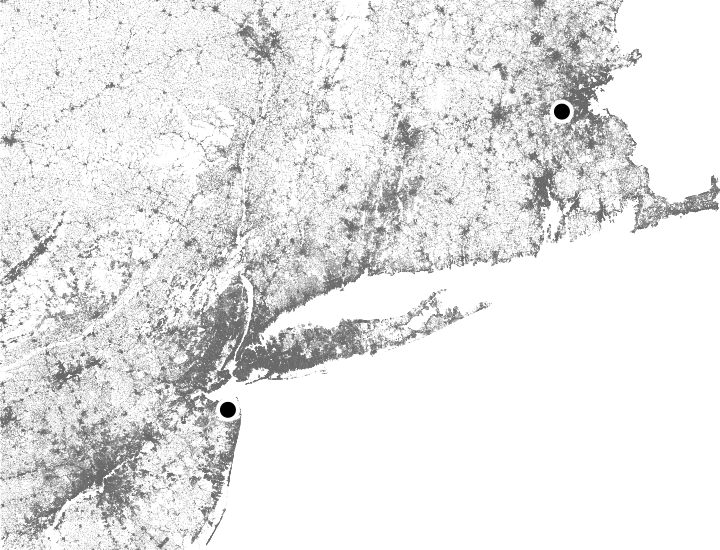
\includegraphics[width=3.5cm]{figs/incbi-road-ne/singleshot/example-intro.png}};
         \coordinate (s) at (1.226,0.63);
         \coordinate (t) at (2.751,1.96);
         \node (slab) at (1.75,0.42) {$s$};
         \node (tlab) at (2.8,1.05) {$t$};
         \draw[->,thick] (slab) -- (s);
         \draw[->,thick] (tlab) -- (t);
      \end{scope}

      \only<2->{
         \node at (2,2.5) {\includegraphics[width=3.5cm]{build/ibid-intro-focus-heuristic}};
         \node at (2,3.8) {Heuristic Search};
      }

      \only<3->{
         \node at (6,2.5) {\includegraphics[width=3.5cm]{build/ibid-intro-focus-bidirectional}};
         \node at (6,3.8) {Bidirectional Search};
      }

      \only<4->{
         \node at (10,2.5) {\includegraphics[width=3.5cm]{build/ibid-intro-focus-incremental}};
         \node at (10,3.8) {Incremental Search};
      }
   
   \end{tikzpicture}
\end{frame}

\begin{frame}
   \frametitle{Outline of Selected Algorithms}
   \begin{tikzpicture}[font=\small]
      \tikzset{>=latex} % arrow heads
      \draw[step=1,black!15,very thin,opacity=\gridopacity] (0,0) grid (12,8);

      \node at (2,6.3) {\includegraphics[width=3.5cm]{build/ibid-intro-focus-heuristic}};
      \node at (2,7.6) {Heuristic Search};
      
      \node at (6,6.3) {\includegraphics[width=3.5cm]{build/ibid-intro-focus-bidirectional}};
      \node at (6,7.6) {Bidirectional Search};
      
      \node at (10,6.3) {\includegraphics[width=3.5cm]{build/ibid-intro-focus-incremental}};
      \node at (10,7.6) {Incremental Search};

      \only<2->{
      \node[inner sep=0pt,anchor=north] at (6,5.0) {\begin{minipage}{9.05cm}
         \begin{tabular}{ccc}
            \toprule
            & Complete & {\only<-4>{\color{white}}Incremental} \\
            \midrule
            \addlinespace[0.2em]
            \strut {\only<-2>{\color{white}}Unidirectional}
               & {\only<-2>{\color{white}}Dijkstra's Algorithm}
               & {\only<-4>{\color{white}}DynamicSWSF-FP} \\
            \addlinespace[-0.2em]
            \strut {\only<-3>{\color{white}}\only<9-10>{\color{gray}}\emph{(Heuristic)}}
               & {\only<-3>{\color{white}}\only<9-10>{\color{gray}}\emph{A*}}
               & {\only<-4>{\color{white}}\only<9-10>{\color{gray}}\emph{Lifelong Planning A*}} \\
            \addlinespace[0.3em]
            \strut {\only<-5>{\color{white}}\only<9-10>{\color{gray}}Bidirectional}
               & {\only<-5>{\color{white}}\only<9-10>{\color{gray}}Bidirectional Dijkstra}
               & \multirow{2}{*}{\large\only<-6>{\color{white}}\only<9-10>{\color{gray}}?} \\
            \addlinespace[-0.2em]
            \strut {\only<-5>{\color{white}}\only<9-10>{\color{gray}}\emph{(Heuristic)}}
               & {\only<-5>{\color{white}}\only<9-10>{\color{gray}}\emph{Bidirectional A*}}
               & \\
            \addlinespace[0.2em]
            \bottomrule
         \end{tabular}
      \end{minipage}};
      }

      \only<8-10>{
      \node[inner sep=0pt,anchor=north] at (6,2.3) {\begin{minipage}{10.2cm}
         {\bf 3 Key Insights:}
         \begin{itemize}
         \item {\only<8-9>{\color{gray}}
            Complete and Incremental methods both create a \emph{trust region (TR)}}
         \item {\color{gray}
            Bidirectional termination can be rewritten w.r.t. edges between TRs}
         \item {\color{gray}
            Heuristic search is equivalent to search over a transformed graph}
         \end{itemize}
      \end{minipage}};
      }

   \end{tikzpicture}
\end{frame}

\begin{frame}
   \frametitle{Distance Functions}
   \begin{tikzpicture}[font=\small]
      \tikzset{>=latex} % arrow heads
      \draw[step=1,black!15,very thin,opacity=\gridopacity] (0,0) grid (12,8);

      \begin{scope}[shift={(4.25,5.2)}]
         \node[inner sep=0pt,anchor=south west] {%
            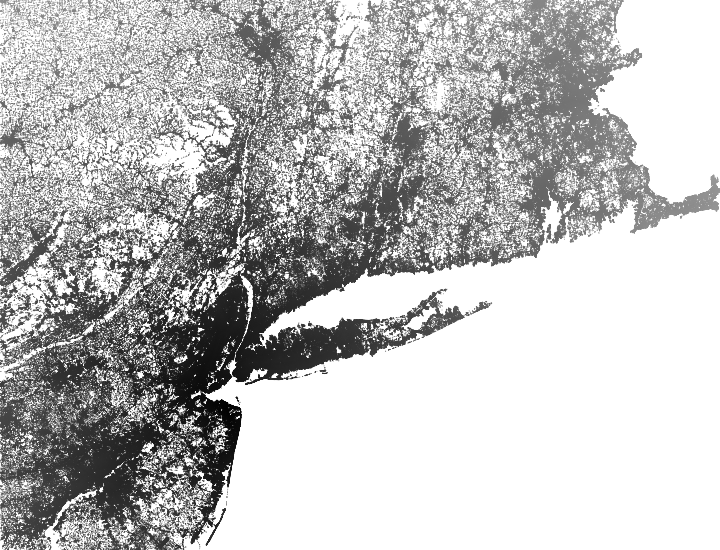
\includegraphics[width=3.5cm]{figs/incbi-road-ne/singleshot/example-dijkstraall.png}};
         \coordinate (s) at (1.226,0.63);
         %\coordinate (t) at (2.751,1.96);
         \node (slab) at (1.75,0.42) {$s$};
         %\node (tlab) at (2.8,1.05) {$t$};
         \draw[->,thick] (slab) -- (s);
         %\draw[->,thick] (tlab) -- (t);
      \end{scope}

      \node[fill=blue!10] at (3,4.0) {\begin{minipage}{5.5cm}
         Definition:
         \[
            d^*(v) = \min_{p \in P_{sv}} \mbox{len}(p,w)
         \]
      \end{minipage}};
      \node[fill=blue!10] at (9,4.0) {\begin{minipage}{5.5cm}
         Local characterization:
         \[
            \arraycolsep=1.4pt
            d^*(v) = 
            \left\{ \begin{array}{cl}
               0 & v = s \\
               \displaystyle\min_{e_{uv}} d^*(u)\!+\!w(e_{uv}) & v \neq s \\
            \end{array} \right.
         \]
      \end{minipage}};

      

      %\only<2->{
      %\node at (6,3.3) {Key: Understanding properties of an approximation $d$.};
      %}

      \only<2->{
      \node[fill=blue!10,minimum width=2cm,align=center] (d) at (6,1.75)
         {Approximation\\$d : V \rightarrow \mathbb{R}$};
      }

      \only<3->{
         \node[align=center] at (6,0.75) {Properties of $d$?};
      }

      \only<4->{
      \node[draw=black!50,densely dashed,minimum width=2cm,align=center] (dprime) at (9,1.75)
         {Approximation\\$d\:\!' : V \rightarrow \mathbb{R}$};
      \draw[->,very thick] (d) -- (dprime);
      }

   \end{tikzpicture}
\end{frame}

\begin{frame}
   \frametitle{Approximating the Distance Function: Complete}
   \begin{tikzpicture}[font=\small]
      \tikzset{>=latex} % arrow heads
      \draw[step=1,black!15,very thin,opacity=\gridopacity] (0,0) grid (12,8);

      \node[fill=blue!10] at (3,7.0) {\begin{minipage}{5.5cm}
         Definition:
         \[
            d^*(v) = \min_{p \in P_{sv}} \mbox{len}(p,w)
         \]
      \end{minipage}};
      \node[fill=blue!10] at (9,7.0) {\begin{minipage}{5.5cm}
         Local characterization:
         \[
            \arraycolsep=1.4pt
            d^*(v) = 
            \left\{ \begin{array}{cl}
               0 & v = s \\
               \displaystyle\min_{e_{uv}} d^*(u)\!+\!w(e_{uv}) & v \neq s \\
            \end{array} \right.
         \]
      \end{minipage}};

      \only<2->{
      \node[fill=black!5,minimum width=5.75cm] at (3,5.5) {\strut Complete Search};
      \node[fill=blue!10,align=center] at (1,4.6) {Fixed\\$w \geq 0$};
      }
      \only<3->{
      \node[fill=blue!10,align=center] at (3.5,4.6) {Approximation\\$d : V \rightarrow \mathbb{R}$};
      }
      \only<4->{
      \node[fill=blue!10,minimum width=5.75cm,minimum height=2.5cm,anchor=north] (tens) at (3,4.0) {};
      \only<7->{
      \node[fill=red!20,minimum width=5.75cm,minimum height=0.5cm] at (3,1.75) {};
      }
      \node[anchor=north] at (tens.north) {\begin{minipage}{5.5cm}
         Constraints on $d$:
         \vspace{-0.2cm}
         \[
             d^*(v) \leq d(v)
         \]
         \vspace{-0.6cm}
         \[
             d(s) = 0
         \]
         \vspace{-0.5cm}
         \[
            \min_{e_{uv}} d(u) + w(e_{uv}) \leq d(v) \quad v \neq s
         \]
         \vspace{-0.3cm}
         \[
            d(u) + w(e_{uv}) \geq d(v)
         \]
         %Ordering, Early Term if $w \geq 0$
      \end{minipage}};
      }

      \only<5>{
         \node[fill=blue!10] (equal) at (9,2.7) {$d = d^*$};
         \draw[->,very thick] (tens) -- (equal);
      }

      % trust region
      \only<6->{
         \node at (9,3.7) {\includegraphics[width=4.5cm]{build/ibid-dijkstra-trust-build,init}};
      }
      \only<8->{
         \node at (9,3.7) {\includegraphics[width=4.5cm]{build/ibid-dijkstra-trust-build,wtensioned}};
      }
      \only<9->{
         \node at (9,3.7) {\includegraphics[width=4.5cm]{build/ibid-dijkstra-trust-build,wtrust}};
      }

      \only<10->{
      \node[fill=blue!10,align=center] at (3,0.7) {
         TR: If $w \geq 0$ and $D$ is the minimal\\
         $d(u)$ among tensioned edges $e_{uv}$,\\
         then any $v$ with $d(v) \leq D$ is correct.
      };
      }

      \only<11->{
         \node[fill=green!10,align=center] at (7.7,0.75) {Relaxation\\Ordering!};
      }
      \only<12->{
         \node[fill=green!10,align=center] at (10.3,0.75) {Early\\Termination!};
      }

   \end{tikzpicture}
\end{frame}

\begin{frame}
   \frametitle{Approximating the Distance Function: Incremental}
   \begin{tikzpicture}[font=\small]
      \tikzset{>=latex} % arrow heads
      \draw[step=1,black!15,very thin,opacity=\gridopacity] (0,0) grid (12,8);

      \node[fill=blue!10] at (3,7.0) {\begin{minipage}{5.5cm}
         Definition:
         \[
            d^*(v) = \min_{p \in P_{sv}} \mbox{len}(p,w)
         \]
      \end{minipage}};
      \node[fill=blue!10] at (9,7.0) {\begin{minipage}{5.5cm}
         Local characterization:
         \[
            \arraycolsep=1.4pt
            d^*(v) = 
            \left\{ \begin{array}{cl}
               0 & v = s \\
               \displaystyle\min_{e_{uv}} d^*(u)\!+\!w(e_{uv}) & v \neq s \\
            \end{array} \right.
         \]
      \end{minipage}};

      \only<-5>{
      \node[fill=black!5,minimum width=5.75cm] at (3,5.5) {\strut Complete Search};
      \node[fill=blue!10,align=center] at (1,4.6) {Fixed\\$w \geq 0$};
      \node[fill=blue!10,align=center] at (3.5,4.6) {Approximation\\$d : V \rightarrow \mathbb{R}$};
      \node[fill=blue!10,minimum width=5.75cm,minimum height=2.5cm,anchor=north] (tens) at (3,4.0) {};
      \node[fill=red!20,minimum width=5.75cm,minimum height=0.5cm] at (3,1.75) {};
      \node[anchor=north] at (tens.north) {\begin{minipage}{5.5cm}
         Constraints on $d$:
         \vspace{-0.2cm}
         \[
             d^*(v) \leq d(v)
         \]
         \vspace{-0.6cm}
         \[
             d(s) = 0
         \]
         \vspace{-0.5cm}
         \[
            \min_{e_{uv}} d(u) + w(e_{uv}) \leq d(v) \quad v \neq s
         \]
         \vspace{-0.3cm}
         \[
            d(u) + w(e_{uv}) \geq d(v)
         \]
         %Ordering, Early Term if $w \geq 0$
      \end{minipage}};
      \fill[white,opacity=0.5] (0,1) rectangle (6,6);
      }

      \node[fill=black!5,minimum width=5.75cm] at (9,5.5) {\strut Incremental Search};

      \only<2->{
      \node[fill=blue!10,align=center] at (7,4.6) {Dynamic\\$w > 0$};
      \node[fill=blue!10,align=center] at (9.5,4.6) {Approximation\\$d : V \rightarrow \mathbb{R}$};
      }

      \only<3-4>{
      \node[fill=blue!10,minimum width=5.75cm,minimum height=2.5cm,anchor=north] (incons) at (9,4.0) {};
      \node[fill=red!20,minimum width=5.75cm,minimum height=0.5cm] at (9,1.75) {};
      \node[anchor=north] at (incons.north) {\begin{minipage}{5.5cm}
         Constraints on $d$:
         \vspace{-0.2cm}
         \[
             d^*(v) \leq d(v)
         \]
         \vspace{-0.6cm}
         \[
             d(s) = 0
         \]
         \vspace{-0.5cm}
         \[
            \min_{e_{uv}} d(u) + w(e_{uv}) \leq d(v) \quad v \neq s
         \]
         \vspace{-0.3cm}
         \[
            d(u) + w(e_{uv}) \geq d(v)
         \]
         %Ordering, Early Term if $w \geq 0$
      \end{minipage}};
      }
      \only<4>{
         \draw[red,ultra thick] (9,3.25) ellipse (1cm and 0.5cm);
         \draw[red,ultra thick] (8.2,3.55) -- (9.8,2.95);
         \draw[red,ultra thick] (8.2,2.95) -- (9.8,3.55);
      }

      \only<5->{
      \node[fill=blue!10,minimum width=5.75cm,minimum height=2.0cm,anchor=north] (incons) at (9,4.0) {};
      \only<7->{
      \node[fill=red!20,minimum width=5.75cm,minimum height=0.5cm] at (9,2.25) {};
      }
      \node[anchor=north] at (incons.north) {\begin{minipage}{5.5cm}
         Constraints on $d$:
         \vspace{-0.2cm}
         \[
            \arraycolsep=1.4pt
            r(v) = 
            \left\{ \begin{array}{cl}
               0 & v = s \\
               \displaystyle\min_{e_{uv}} d(u)\!+\!w(e_{uv}) & v \neq s \\
            \end{array} \right.
         \]
         \vspace{-0.3cm}
         \[
             d(v) = r(v)
         \]
         %Ordering, Early Term if $w \geq 0$
      \end{minipage}};
      }

      \only<6-7>{
         \node at (3,3.7) {\includegraphics[width=4.5cm]{build/ibid-dijkstra-trust-build,init}};
      }
      \only<8>{
         \node at (3,3.7) {\includegraphics[width=4.5cm]{build/ibid-dijkstra-trust-build,wincons}};
      }
      \only<9->{
         \node at (3,3.7) {\includegraphics[width=4.5cm]{build/ibid-dijkstra-trust-build,winctrust}};
      }
      
      \only<10->{
      \node[fill=blue!10,align=center] at (9,1.0) {
         TR: If $w > 0$ and $K$ is the minimal \\
         $k(v) = \min(d(v), r(v))$ among $V_{\ms{incons}}$, \\
         then any consistent $v$ \\
         with $d(v) \leq K$ is correct.
      };
      }

      \only<11->{
         \node[fill=green!10,align=center] at (1.7,0.75) {Relaxation\\Ordering!};
         \node[fill=green!10,align=center] at (4.3,0.75) {Early\\Termination!};
      }

   \end{tikzpicture}
\end{frame}

\begin{frame}
   \frametitle{Complete/Incremental Trust Regions}
   \begin{tikzpicture}[font=\small]
      \tikzset{>=latex} % arrow heads
      \draw[step=1,black!15,very thin,opacity=\gridopacity] (0,0) grid (12,8);


      % complete side
      \node[fill=black!5,minimum width=5.75cm] at (3,7.5) {\strut Complete Search};
      \node[fill=blue!10,align=center] at (1,6.6) {Fixed\\$w \geq 0$};
      \node[fill=blue!10,align=center] at (3.5,6.6) {Approximation\\$d : V \rightarrow \mathbb{R}$};
      \node[fill=blue!10,minimum width=5.75cm,minimum height=2.5cm,anchor=north] (tens) at (3,6.0) {};
      \node[fill=red!20,minimum width=5.75cm,minimum height=0.5cm] at (3,3.75) {};
      \node[anchor=north] at (tens.north) {\begin{minipage}{5.5cm}
         Constraints on $d$:
         \vspace{-0.2cm}
         \[
             d^*(v) \leq d(v)
         \]
         \vspace{-0.6cm}
         \[
             d(s) = 0
         \]
         \vspace{-0.5cm}
         \[
            \min_{e_{uv}} d(u) + w(e_{uv}) \leq d(v) \quad v \neq s
         \]
         \vspace{-0.3cm}
         \[
            d(u) + w(e_{uv}) \geq d(v)
         \]
         %Ordering, Early Term if $w \geq 0$
      \end{minipage}};
      \node[fill=blue!10,align=center] at (3,2.75) {
         TR: If $w \geq 0$ and $D$ is the minimal\\
         $d(u)$ among tensioned edges $e_{uv}$,\\
         then any $v$ with $d(v) \leq D$ is correct.
      };
      \node at (3,1.05) {\includegraphics[width=2.5cm]{build/ibid-dijkstra-trust-build,wtrust}};

      % incremental side
      \node[fill=black!5,minimum width=5.75cm] at (9,7.5) {\strut Incremental Search};
      \node[fill=blue!10,align=center] at (7,6.6) {Dynamic\\$w > 0$};
      \node[fill=blue!10,align=center] at (9.5,6.6) {Approximation\\$d : V \rightarrow \mathbb{R}$};
      \node[fill=blue!10,minimum width=5.75cm,minimum height=2.0cm,anchor=north] (incons) at (9,6.0) {};
      \node[fill=red!20,minimum width=5.75cm,minimum height=0.5cm] at (9,4.25) {};
      \node[anchor=north] at (incons.north) {\begin{minipage}{5.5cm}
         Constraints on $d$:
         \vspace{-0.2cm}
         \[
            \arraycolsep=1.4pt
            r(v) = 
            \left\{ \begin{array}{cl}
               0 & v = s \\
               \displaystyle\min_{e_{uv}} d(u)\!+\!w(e_{uv}) & v \neq s \\
            \end{array} \right.
         \]
         \vspace{-0.3cm}
         \[
             d(v) = r(v)
         \]
         %Ordering, Early Term if $w \geq 0$
      \end{minipage}};
      \node[fill=blue!10,align=center] at (9,3.0) {
         TR: If $w > 0$ and $K$ is the minimal \\
         $k(v) = \min(d(v), r(v))$ among $V_{\ms{incons}}$, \\
         then any consistent $v$ \\
         with $d(v) \leq K$ is correct.
      };
      \node at (9,1.05) {\includegraphics[width=2.5cm]{build/ibid-dijkstra-trust-build,winctrust}};

   \end{tikzpicture}
\end{frame}

%\begin{frame}
%   \frametitle{Trust Regions}
%   \begin{tikzpicture}[font=\small]
%      \tikzset{>=latex} % arrow heads
%      \draw[step=1,black!15,very thin,opacity=\gridopacity] (0,0) grid (12,8);
%
%      % ordering problems
%      %\begin{scope}[shift={(1.5,5.5)}]
%      %\begin{scope}[shift={(0,0)}]
%      %   \node[fill=black,circle,inner sep=1.2pt] (a) at (0,0) {};
%      %   \node[fill=black,circle,inner sep=1.2pt] (b) at (1.5,0) {};
%      %   \node[fill=black,circle,inner sep=1.2pt] (c) at (3.0,0) {};
%      %   \draw[->,densely dashed] (a) -- (b) node[midway,fill=white,circle,inner sep=1pt] {1};
%      %   \draw[->,densely dashed] (b) -- (c) node[midway,fill=white,circle,inner sep=1pt] {1};
%      %   
%      %   \node[above=-0.00cm of a] {$a$};
%      %   \node[above=-0.00cm of b] {$b$};
%      %   \node[above=-0.00cm of c] {$c$};
%      %
%      %   \node[below=0.05cm of a] {$d=0$};
%      %   \node[below=0.05cm of b] {$d=2$};
%      %   \node[below=0.05cm of c] {$d=4$};
%      %\end{scope}
%      %
%      %\begin{scope}[shift={(0,-1)}]
%      %   \node[fill=black,circle,inner sep=1.2pt] (a) at (0,0) {};
%      %   \node[fill=black,circle,inner sep=1.2pt] (b) at (1.5,0) {};
%      %   \node[fill=black,circle,inner sep=1.2pt] (c) at (3.0,0) {};
%      %   \draw[->,densely dashed] (a) -- (b) node[midway,fill=white,circle,inner sep=1pt] {1};
%      %   \draw[line width=0.10cm,black!10] (b) -- (c) node[midway,fill=white,circle,inner sep=1pt] {1};
%      %   \draw[->] (b) -- (c) node[midway,fill=white,circle,inner sep=1pt] {1};
%      %
%      %   \node[below=0.05cm of a] {$d=0$};
%      %   \node[below=0.05cm of b] {$d=2$};
%      %   \node[below=0.05cm of c] {$d=3$};
%      %\end{scope}
%      %
%      %\begin{scope}[shift={(0,-2)}]
%      %   \node[fill=black,circle,inner sep=1.2pt] (a) at (0,0) {};
%      %   \node[fill=black,circle,inner sep=1.2pt] (b) at (1.5,0) {};
%      %   \node[fill=black,circle,inner sep=1.2pt] (c) at (3.0,0) {};
%      %   \draw[line width=0.10cm,black!10] (a) -- (b) node[midway,fill=white,circle,inner sep=1pt] {1};
%      %   \draw[->] (a) -- (b) node[midway,fill=white,circle,inner sep=1pt] {1};
%      %   \draw[->,densely dashed] (b) -- (c) node[midway,fill=white,circle,inner sep=1pt] {1};
%      %   
%      %   \node[below=0.05cm of a] {$d=0$};
%      %   \node[below=0.05cm of b] {$d=1$};
%      %   \node[below=0.05cm of c] {$d=3$};
%      %\end{scope}
%      %
%      %\begin{scope}[shift={(0,-3)}]
%      %   \node[fill=black,circle,inner sep=1.2pt] (a) at (0,0) {};
%      %   \node[fill=black,circle,inner sep=1.2pt] (b) at (1.5,0) {};
%      %   \node[fill=black,circle,inner sep=1.2pt] (c) at (3.0,0) {};
%      %   \draw[->] (a) -- (b) node[midway,fill=white,circle,inner sep=1pt] {1};
%      %   \draw[line width=0.10cm,black!10] (b) -- (c) node[midway,fill=white,circle,inner sep=1pt] {1};
%      %   \draw[->] (b) -- (c) node[midway,fill=white,circle,inner sep=1pt] {1};
%      %   
%      %   \node[below=0.05cm of a] {$d=0$};
%      %   \node[below=0.05cm of b] {$d=1$};
%      %   \node[below=0.05cm of c] {$d=2$};
%      %\end{scope}
%      %\end{scope}
%
%      \node[fill=blue!10] at (3,7.25) {$d : V \rightarrow \mathbb{R}$};
%
%      \node[fill=blue!10,minimum width=5.75cm,minimum height=3.5cm] (erelax) at (3,5) {};
%      \node[anchor=north] at (erelax.north) {\begin{minipage}{5.5cm}
%         Tensioned Approximation $d$:
%         \vspace{-0.2cm}
%         \[
%             d^*(v) \leq d(v)
%         \]
%         \vspace{-0.6cm}
%         \[
%             d(s) = 0
%         \]
%         \vspace{-0.5cm}
%         \[
%            \min_{e_{uv}} d(u) + w(e_{uv}) \leq d(v)
%         \]
%         \vspace{-0.4cm}
%         \[
%            d(u) + w(e_{uv}) \geq d(v) [RELAXED]
%         \]
%         \only<2->{Ordering, Early Term if $w \geq 0$}
%      \end{minipage}};
%
%      % trust region
%      \node at (9,6.0) {\includegraphics[width=4.5cm]{build/ibid-dijkstra-trust}};
%
%
%      \only<3->{
%      \node[fill=blue!10,align=center] at (5,2.5) {
%         Trust Region:\\
%         If $w \geq 0$ and $D$ is the minimum $d(u)$ among tensioned edges $e_{uv}$,\\
%         then any $v$ with $d(v) \leq D$ is correct.
%      };
%      }
%
%      \only<4->{
%         \node[fill=blue!10,align=center] at (5,1.0) {
%            Algorithm: Order edges by $d(u)$ (Dijkstra's algorithm).
%         };
%
%         \node at (10.9,2.9) {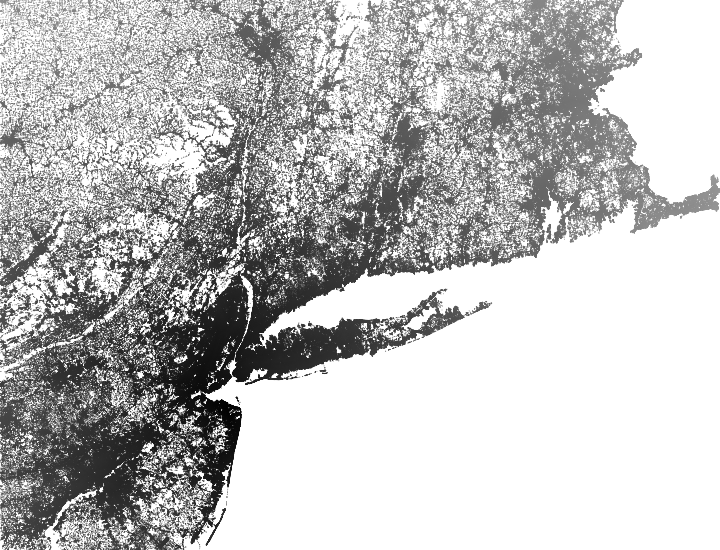
\includegraphics[width=2cm]{figs/incbi-road-ne/singleshot/example-dijkstraall.png}};
%         \node at (10.9,1.1) {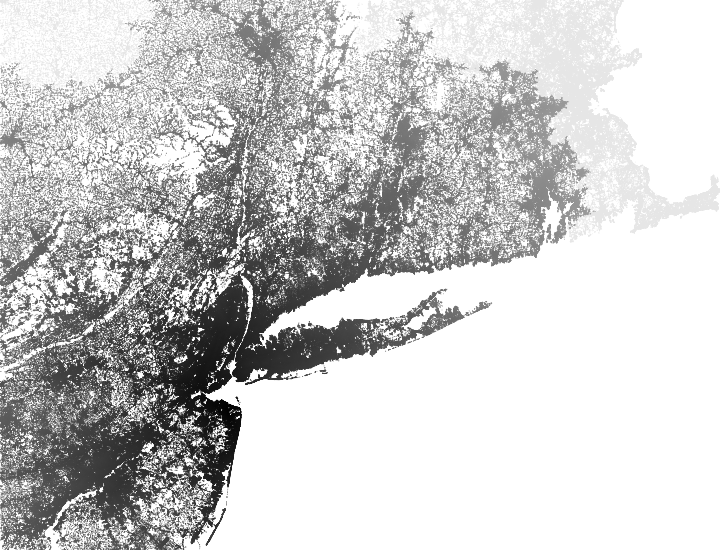
\includegraphics[width=2cm]{figs/incbi-road-ne/singleshot/example-dijkstra.png}};
%
%
%         \node[fill=blue!10,minimum width=5.75cm,minimum height=1.0cm] (erelax) at (3,0.7) {};
%         \node[anchor=north] at (erelax.north) {\begin{minipage}{5.5cm}
%            Terminate when $d(t) \leq D$.
%
%            $p$: Walk backwards on $d$ from $t$.
%         \end{minipage}};
%      }
%      
%   \end{tikzpicture}
%\end{frame}

\begin{frame}
   \frametitle{Outline of Selected Algorithms}
   \begin{tikzpicture}[font=\small]
      \tikzset{>=latex} % arrow heads
      \draw[step=1,black!15,very thin,opacity=\gridopacity] (0,0) grid (12,8);

      \node at (2,6.3) {\includegraphics[width=3.5cm]{build/ibid-intro-focus-heuristic}};
      \node at (2,7.6) {Heuristic Search};
      
      \node at (6,6.3) {\includegraphics[width=3.5cm]{build/ibid-intro-focus-bidirectional}};
      \node at (6,7.6) {Bidirectional Search};
      
      \node at (10,6.3) {\includegraphics[width=3.5cm]{build/ibid-intro-focus-incremental}};
      \node at (10,7.6) {Incremental Search};

      \node[inner sep=0pt,anchor=north] at (6,5.0) {\begin{minipage}{9.05cm}
         \begin{tabular}{ccc}
            \toprule
            & Complete & Incremental \\
            \midrule
            \addlinespace[0.2em]
            \strut Unidirectional
               & Dijkstra's Algorithm
               & DynamicSWSF-FP \\
            \addlinespace[-0.2em]
            \strut {\color{gray}\emph{(Heuristic)}}
               & {\color{gray}\emph{A*}}
               & {\color{gray}\emph{Lifelong Planning A*}} \\
            \addlinespace[0.3em]
            \strut {\only<1>{\color{gray}}Bidirectional}
               & {\only<1>{\color{gray}}Bidirectional Dijkstra}
               & \multirow{2}{*}{\large\color{gray}?} \\
            \addlinespace[-0.2em]
            \strut {\color{gray}\emph{(Heuristic)}}
               & {\color{gray}\emph{Bidirectional A*}}
               & \\
            \addlinespace[0.2em]
            \bottomrule
         \end{tabular}
      \end{minipage}};

      \node[inner sep=0pt,anchor=north] at (6,2.3) {\begin{minipage}{10.2cm}
         {\bf 3 Key Insights:}
         \begin{itemize}
         \item Complete and Incremental methods both create a \emph{trust region (TR)}
         \item {\only<1-2>{\color{gray}}\only<1-3>{}
            Bidirectional termination can be rewritten w.r.t. edges between TRs}
         \item {\color{gray}
            Heuristic search is equivalent to search over a transformed graph}
         \end{itemize}
      \end{minipage}};

   \end{tikzpicture}
\end{frame}

\begin{frame}
   \frametitle{Bidirectional Search: Termination Condition}
   \begin{tikzpicture}[font=\small]
      \tikzset{>=latex} % arrow heads
      \draw[step=1,black!15,very thin,opacity=\gridopacity] (0,0) grid (12,8);

      \only<1>{\node at (6.0,5.8) {\includegraphics{build/ibid-bidijkstra-viz-build,a}};}
      \only<2>{\node at (6.0,5.8) {\includegraphics{build/ibid-bidijkstra-viz-build,b}};}
      \only<3>{\node at (6.0,5.8) {\includegraphics{build/ibid-bidijkstra-viz-build,c}};}
      \only<4>{\node at (6.0,5.8) {\includegraphics{build/ibid-bidijkstra-viz-build,d}};}
      \only<5>{\node at (6.0,5.8) {\includegraphics{build/ibid-bidijkstra-viz-build,e}};}
      \only<6-7>{\node at (6.0,5.8) {\includegraphics{build/ibid-bidijkstra-viz-build,f}};}
      \only<8->{\node at (6.0,5.8) {\includegraphics{build/ibid-bidijkstra-viz-build,g}};}

      \only<1-9>{
      \node[anchor=north] at (6,3.7) {\begin{minipage}{9.5cm}
         \begin{algorithmic}[1]
         \Procedure{BidirectionalTerminationA}{}
         \State Build approximations $d_s$ and $d_t$ (alternate arbitrarily).
         \State Stop on first vertex $x$ CLOSED by both sides.
         \State Return path by walking $d_s$ from $x$ to $s$
            and $d_t$ from $x$ to $t$.
         \EndProcedure
         \end{algorithmic}
      \end{minipage}};
      }
      \only<10-12>{
      \node[anchor=north] at (6,3.7) {\begin{minipage}{9.5cm}
         \begin{algorithmic}[1]
         \Procedure{BidirectionalTerminationB}{}
         \State $p_{\ms{sofar}} \leftarrow$ best path found so far.
         \State Build approximations $d_s$ and $d_t$ (alternate arbitrarily).
         \State When $s$-expanding $u$, if edge $e_{uv}$ has $v$ is in CLOSED$_t$,
         \State \qquad Update $p_{\ms{sofar}}$ if $d_s(u) + w(e_{uv}) + d_t(v)$ is better.
         \State (Do the same in the reverse direction.)
         \State Stop on first vertex $x$ CLOSED by both sides.
         \State Return path $p_{\ms{sofar}}$.
         \EndProcedure
         \end{algorithmic}
      \end{minipage}};
      }
      \only<13->{
      \node[anchor=north] at (6,3.7) {\begin{minipage}{9.5cm}
         \definecolor{greenhighlight}{rgb}{0.8, 1.0, 0.8}
         \begin{algorithmic}[1]
         \Procedure{BidirectionalTerminationB}{}
         \State $p_{\ms{sofar}} \leftarrow$ best path found so far.
         \State Build approximations $d_s$ and $d_t$ (alternate arbitrarily).
         \State When $s$-expanding $u$, if edge $e_{uv}$ has $v$ is in CLOSED$_t$,
         \State \qquad Update $p_{\ms{sofar}}$ if $d_s(u) + w(e_{uv}) + d_t(v)$ is better.
         \State (Do the same in the reverse direction.)
         \State \colorbox{greenhighlight}{Stop on when $\mbox{len}(p_{\ms{sofar}}) \leq D_s + D_t$.}
         \State Return path $p_{\ms{sofar}}$.
         \EndProcedure
         \end{algorithmic}
      \end{minipage}};
      }

      \only<7-9>{\node[color=red,draw,anchor=west] at (6,1.5) {\strut Unsound!};}
      \only<11>{\node[color=green!50!black,draw,anchor=west] at (6,0.4) {\strut Correct};}
      \only<12>{\node[color=green!50!black,draw,anchor=west] at (6,0.4) {\strut Correct, {\color{red} but overconservative.}};}

      % from illustration of bidirectional termination problem!
      \only<9>{
      \fill[white,opacity=0.9] (2,3.6) rectangle (10,7.9);
      \node[fill=blue!5,rounded corners,minimum width=6cm,minimum height=2.5cm] at (6.0,5.8) {};
      \begin{scope}[shift={(3.75,5.4)}]
         \node[fill=black,circle,inner sep=1.2pt] (s) at (0,0) {};
         \node[fill=black,circle,inner sep=1.2pt] (a) at (1.5,0) {};
         \node[fill=black,circle,inner sep=1.2pt] (b) at (3.0,0) {};
         \node[fill=black,circle,inner sep=1.2pt] (t) at (4.5,0) {};
         \node[fill=black,circle,inner sep=1.2pt] (c) at (2.25,0.8) {};
         \draw[->] (s) -- (a) node[midway,fill=blue!5,circle,inner sep=1pt] {3};
         \draw[->] (a) -- (b) node[midway,fill=blue!5,circle,inner sep=1pt] {3};
         \draw[->] (b) -- (t) node[midway,fill=blue!5,circle,inner sep=1pt] {3};
         \draw[->] (a) -- (c) node[midway,fill=blue!5,circle,inner sep=1pt] {2};
         \draw[->] (c) -- (b) node[midway,fill=blue!5,circle,inner sep=1pt] {2};
         \node[below=0.07cm of s] {$s$};
         \node[below=0.07cm of a] {$a$};
         \node[below=0.07cm of b] {$b$};
         \node[below=0.07cm of t] {$t$};
         \node[above=0.07cm of c] {$c$};

         % represent closed sets
         \node[fill=blue,circle,inner sep=1.2pt,below left=0.05cm of s] {};
         \node[fill=blue,circle,inner sep=1.2pt,below left=0.05cm of a] {};
         \node[draw=blue,circle,inner sep=1.2pt,below left=0.05cm of b] {};
         \node[fill=blue,circle,inner sep=1.2pt,above left=0.05cm of c] {};

         \node[fill=red,circle,inner sep=1.2pt,below right=0.05cm of t] {};
         \node[fill=red,circle,inner sep=1.2pt,above right=0.05cm of c] {};
         \node[draw=red,circle,inner sep=1.2pt,below right=0.05cm of a] {};
         \node[fill=red,circle,inner sep=1.2pt,below right=0.05cm of b] {};
      \end{scope}
      }

      % other example
      \only<14>{
      \fill[white,opacity=0.9] (2,3.6) rectangle (10,7.9);
      \node[fill=blue!5,rounded corners,minimum width=6cm,minimum height=2.5cm] at (6.0,5.8) {};
      \begin{scope}[shift={(3.75,5.4)}]
         \node[fill=black,circle,inner sep=1.2pt] (s) at (0,0) {};
         \node[fill=black,circle,inner sep=1.2pt] (a) at (1.5,0) {};
         \node[fill=black,circle,inner sep=1.2pt] (b) at (3.0,0) {};
         \node[fill=black,circle,inner sep=1.2pt] (t) at (4.5,0) {};
         \node[fill=black,circle,inner sep=1.2pt] (c) at (1.5,0.8) {};
         \node[fill=black,circle,inner sep=1.2pt] (d) at (3.0,0.8) {};
         \draw[->] (s) -- (a) node[midway,fill=white,circle,inner sep=1pt] {3};
         \draw[->] (a) -- (b) node[midway,fill=white,circle,inner sep=1pt] {3};
         \draw[->] (b) -- (t) node[midway,fill=white,circle,inner sep=1pt] {3};
         \draw[->] (a) -- (c) node[midway,fill=white,circle,inner sep=1pt] {2};
         \draw[->] (d) -- (b) node[midway,fill=white,circle,inner sep=1pt] {2};
         \node[below=0.07cm of s] {$s$};
         \node[below=0.07cm of a] {$a$};
         \node[below=0.07cm of b] {$b$};
         \node[below=0.07cm of t] {$t$};
         \node[above=0.07cm of c] {$c$};
         \node[above=0.07cm of d] {$d$};

         % represent closed sets
         \node[fill=blue,circle,inner sep=1.2pt,below left=0.05cm of s] {};
         \node[fill=blue,circle,inner sep=1.2pt,below left=0.05cm of a] {};
         \node[draw=blue,circle,inner sep=1.2pt,below left=0.05cm of b] {};
         \node[fill=blue,circle,inner sep=1.2pt,above left=0.05cm of c] {};

         \node[fill=red,circle,inner sep=1.2pt,below right=0.05cm of t] {};
         \node[fill=red,circle,inner sep=1.2pt,above right=0.05cm of d] {};
         \node[draw=red,circle,inner sep=1.2pt,below right=0.05cm of a] {};
         \node[fill=red,circle,inner sep=1.2pt,below right=0.05cm of b] {};
      \end{scope}
      }

      \node[inner sep=0pt,anchor=south east] at (11.9,0.1) {\scriptsize Amoebas!};

   \end{tikzpicture}
\end{frame}

\begin{frame}
   \frametitle{Bidirectional Search: Terminating with Trust Regions}
   \begin{tikzpicture}[font=\small]
      \tikzset{>=latex} % arrow heads
      \draw[step=1,black!15,very thin,opacity=\gridopacity] (0,0) grid (12,8);

      \node[anchor=north] at (6,7.5) {\begin{minipage}{9.5cm}
         \definecolor{greenhighlight}{rgb}{0.8, 1.0, 0.8}
         \begin{algorithmic}[1]
         \Procedure{BidirectionalTerminationB}{}
         \State $p_{\ms{sofar}} \leftarrow$ best path found so far.
         \State Build approximations $d_s$ and $d_t$ (alternate arbitrarily).
         \State When $s$-expanding $u$, if edge $e_{uv}$ has $v$ is in CLOSED$_t$,
         \State \qquad Update $p_{\ms{sofar}}$ if $d_s(u) + w(e_{uv}) + d_t(v)$ is better.
         \State (Do the same in the reverse direction.)
         \State Stop on when $\mbox{len}(p_{\ms{sofar}}) \leq D_s + D_t$.
         \State Return path $p_{\ms{sofar}}$.
         \EndProcedure
         \end{algorithmic}
      \end{minipage}};

      \only<2>{
      \draw[->,thick] (6,4.0) -- (6,3.1);
      \node[fill=blue!10] at (6,2.0) {\begin{minipage}{11cm}
         Define $E_{\ms{conn}}$ as the set of all edges $e_{uv}$ such that
         $d_s(u) \leq D_s$ and $d_t(v) \leq D_t$,
         and define $\ell_e$ s.t. $\ell_e(e_{uv}) = d_s(u) + w(e_{uv}) + d_t(v)$.
         If $w \geq 0$,
         $s \neq t$,
         $E_{\ms{conn}}$ is non-empty,
         and $e^*_{uv}$ minimizes $\ell_e$
         among $E_{\ms{conn}}$ with $\ell_e(e^*_{uv}) \leq D_s + D_t$,
         then $\ell_e(e^*_{uv})$ is the length of a shortest path,
         and $e^*_{uv}$ lies on one such path.
      \end{minipage}};
      }
      
   \end{tikzpicture}
\end{frame}

\begin{frame}
   \frametitle{Outline of Selected Algorithms}
   \begin{tikzpicture}[font=\small]
      \tikzset{>=latex} % arrow heads
      \draw[step=1,black!15,very thin,opacity=\gridopacity] (0,0) grid (12,8);

      \node at (2,6.3) {\includegraphics[width=3.5cm]{build/ibid-intro-focus-heuristic}};
      \node at (2,7.6) {Heuristic Search};
      
      \node at (6,6.3) {\includegraphics[width=3.5cm]{build/ibid-intro-focus-bidirectional}};
      \node at (6,7.6) {Bidirectional Search};
      
      \node at (10,6.3) {\includegraphics[width=3.5cm]{build/ibid-intro-focus-incremental}};
      \node at (10,7.6) {Incremental Search};

      \node[inner sep=0pt,anchor=north] at (6,5.0) {\begin{minipage}{9.05cm}
         \begin{tabular}{ccc}
            \toprule
            & Complete & Incremental \\
            \midrule
            \addlinespace[0.2em]
            \strut Unidirectional
               & Dijkstra's Algorithm
               & DynamicSWSF-FP \\
            \addlinespace[-0.2em]
            \strut {\color{gray}\emph{(Heuristic)}}
               & {\color{gray}\emph{A*}}
               & {\color{gray}\emph{Lifelong Planning A*}} \\
            \addlinespace[0.3em]
            \strut Bidirectional
               & Bidirectional Dijkstra
               & \only<1>{\multirow{2}{*}{\large\color{gray}?}}
                 \only<2>{IBiD} \\
            \addlinespace[-0.2em]
            \strut {\color{gray}\emph{(Heuristic)}}
               & {\color{gray}\emph{Bidirectional A*}}
               & \only<2>{\color{gray}?} \\
            \addlinespace[0.2em]
            \bottomrule
         \end{tabular}
      \end{minipage}};

      \node[inner sep=0pt,anchor=north] at (6,2.3) {\begin{minipage}{10.2cm}
         {\bf 3 Key Insights:}
         \begin{itemize}
         \item Complete and Incremental methods both create a \emph{trust region (TR)}
         \item Bidirectional termination can be rewritten w.r.t. edges between TRs
         \item {\color{gray}
            Heuristic search is equivalent to search over a transformed graph}
         \end{itemize}
      \end{minipage}};

   \end{tikzpicture}
\end{frame}

\begin{frame}
   \frametitle{Incremental Bidirectional Dijkatra's Algorithm (IBiD)}
   \begin{tikzpicture}[font=\small]
      \tikzset{>=latex} % arrow heads
      \draw[step=1,black!15,very thin,opacity=\gridopacity] (0,0) grid (12,8);

      \node at (6,5.9) {\includegraphics{build/ibid-bidijkstra-sep}};

      \only<2->{
      \node[fill=blue!5,align=center,minimum width=3.5cm] at (1.8,3.3) {$Q_s$: $d_s$ Inconsistent\\Vertex Queue};
      }
      \only<3->{
      \node[inner sep=0pt,align=center] at (1.8,2.2) {$u$ on $Q_s$ iff:\\$d_s(u)\!\neq\!r_s(u)$};
      }
      \only<4->{
      \node[inner sep=0pt,align=center] at (1.8,1.1) {$Q_s$ sorted by:\\$k_s(u)\!=\!\min(d_s(u),\!r_s(u))$};
      }

      \only<5->{
      \node[fill=red!5,align=center,minimum width=3.5cm] at (10.2,3.3) {$Q_t$: $d_t$ Inconsistent\\Vertex Queue};
      \node[inner sep=0pt,align=center] at (10.2,2.2) {$v$ on $Q_t$ iff:\\$d_t(v)\!\neq\!r_t(v)$};
      \node[inner sep=0pt,align=center] at (10.2,1.1) {$Q_t$ sorted by;\\$k_t(v)\!=\!\min(d_t(v),\!r_t(v))$};
      }

      \only<6->{
      \node[fill=green!10,align=center,minimum width=4.2cm] at (6,3.3) {$Q_c$: Connection\\Edge Queue};
      }
      \only<7->{
      \node[inner sep=0pt,align=center] at (6,2.2) {
         $e_{uv}$ on $Q_c$ iff:\\
         $d_s(u) = r_s(u); \; d_t(v) = r_t(v)$\\
         $d_s(u) \leq K_s; \; d_t(v) \leq K_t$};
      }
      \only<8->{
      \node[inner sep=0pt,align=center] at (6,1.1) {
         $Q_c$ sorted by:\\
         $d_s(u) + w(e_{uv}) + d_t(v)$};
      }
      \only<9->{
      \node[fill=green!15] at (6,0.3) {
         Terminate when $Q_c.\mbox{\sc TopKey} \leq K_s + K_t$.};
      }

   \end{tikzpicture}
\end{frame}

\begin{frame}
   \frametitle{Traffic Problem Results}
   \begin{tikzpicture}[font=\small]
      \tikzset{>=latex} % arrow heads
      \draw[step=1,black!15,very thin,opacity=\gridopacity] (0,0) grid (12,8);

      \node at (3.2,6.4) {\begin{minipage}{6.1cm}
         9th DIMACS Implementation Challenge

         $G$: 1,524,453 vertices and 3,868,020 edges

         \vspace{0.15cm}
         Traffic model:
         \vspace{-0.1cm}
         \begin{itemize}
         \setlength\itemsep{-0.05cm}
         \item Independently blocked edges
         \item $P_{\ms{blocked}} = 0.002$
         \item Transitions: $P_{\ms{block}}: 0.0010 \mbox{ to } 0.0001$
         \item 10 planning episodes
         \end{itemize}
      \end{minipage}};

      \node[draw=black!30,inner sep=0pt] (exdijk) at (1.7,3.7) {
         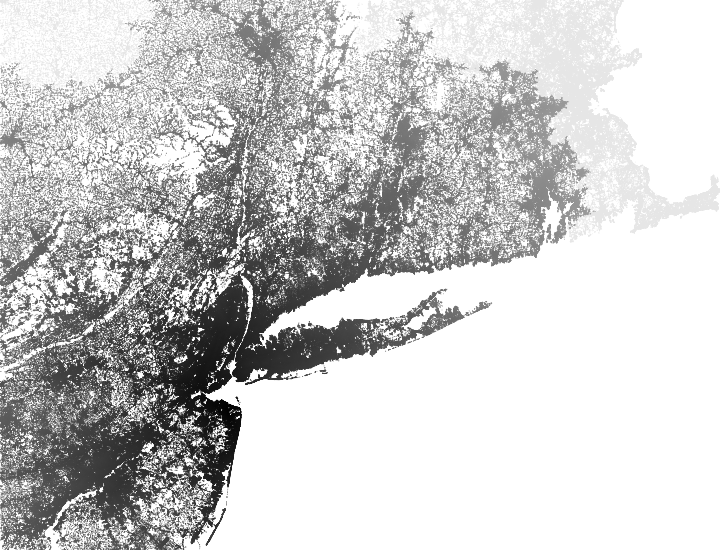
\includegraphics[width=3cm]{figs/incbi-road-ne/singleshot/example-dijkstra.png}};
      \node[draw=black!30,inner sep=0pt] (exdynswsf) at (4.8,3.7) {
         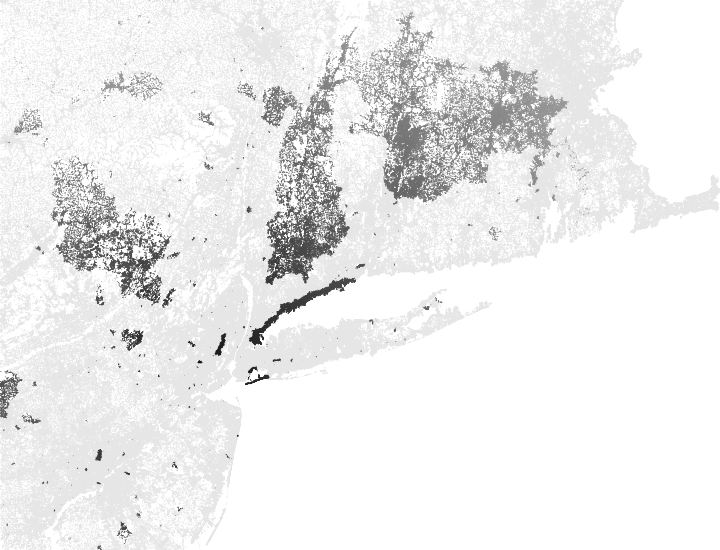
\includegraphics[width=3cm]{figs/incbi-road-ne/singleshot/example-incuni-1.png}};
         
      \node[draw=black!30,inner sep=0pt] (exbidijk) at (1.7,1.3) {
         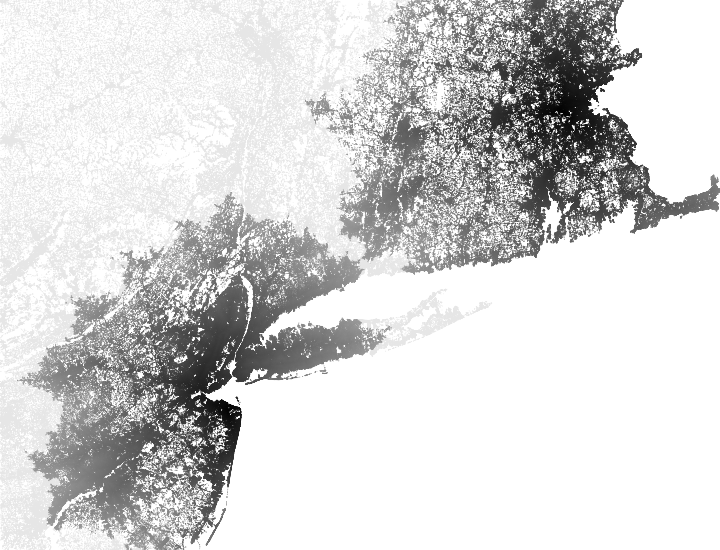
\includegraphics[width=3cm]{figs/incbi-road-ne/singleshot/example-bidijkstra.png}};
      \node[draw=black!30,inner sep=0pt] (exibid) at (4.8,1.3) {
         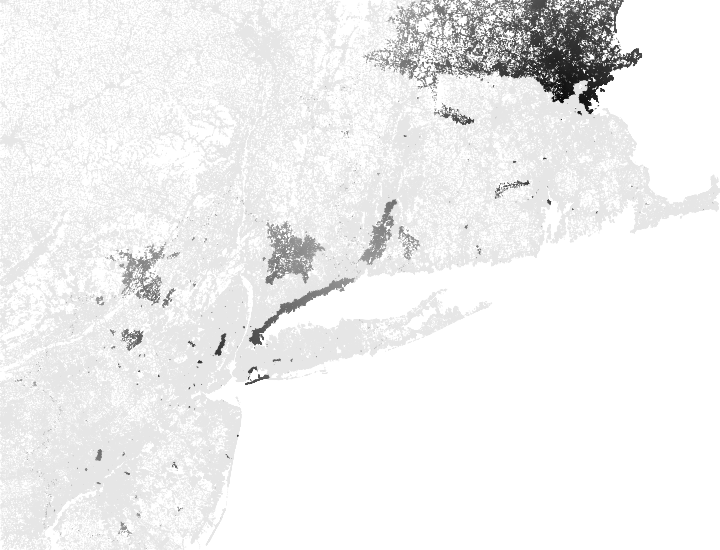
\includegraphics[width=3cm]{figs/incbi-road-ne/singleshot/example-incbi-1.png}};

      \node[anchor=south east] at (exdijk.south east) {Dijk};
      \node[anchor=south east] at (exdynswsf.south east) {DynSWSF};
      \node[anchor=south east] at (exbidijk.south east) {BiDijk};
      \node[anchor=south east] at (exibid.south east) {IBiD};

      \node at (9.2,3.8) {\includegraphics{build/incbi-road-ne/stats2vert-nonheur}};

   \end{tikzpicture}
\end{frame}

\begin{frame}
   \frametitle{Outline of Selected Algorithms}
   \begin{tikzpicture}[font=\small]
      \tikzset{>=latex} % arrow heads
      \draw[step=1,black!15,very thin,opacity=\gridopacity] (0,0) grid (12,8);

      \node at (2,6.3) {\includegraphics[width=3.5cm]{build/ibid-intro-focus-heuristic}};
      \node at (2,7.6) {Heuristic Search};
      
      \node at (6,6.3) {\includegraphics[width=3.5cm]{build/ibid-intro-focus-bidirectional}};
      \node at (6,7.6) {Bidirectional Search};
      
      \node at (10,6.3) {\includegraphics[width=3.5cm]{build/ibid-intro-focus-incremental}};
      \node at (10,7.6) {Incremental Search};

      \node[inner sep=0pt,anchor=north] at (6,5.0) {\begin{minipage}{9.05cm}
         \begin{tabular}{ccc}
            \toprule
            & Complete & Incremental \\
            \midrule
            \addlinespace[0.2em]
            \strut Unidirectional
               & Dijkstra's Algorithm
               & DynamicSWSF-FP \\
            \addlinespace[-0.2em]
            \strut {\only<1>{\color{gray}}\emph{(Heuristic)}}
               & {\only<1>{\color{gray}}\emph{A*}}
               & {\only<1>{\color{gray}}\emph{Lifelong Planning A*}} \\
            \addlinespace[0.3em]
            \strut Bidirectional
               & Bidirectional Dijkstra
               & IBiD \\
            \addlinespace[-0.2em]
            \strut {\only<1>{\color{gray}}\emph{(Heuristic)}}
               & {\only<1>{\color{gray}}\emph{Bidirectional A*}}
               & \only<1>{\color{gray}?}
                 \only<2->{\emph{Heuristic IBiD}} \\
            \addlinespace[0.2em]
            \bottomrule
         \end{tabular}
      \end{minipage}};

      \node[inner sep=0pt,anchor=north] at (6,2.3) {\begin{minipage}{10.2cm}
         {\bf 3 Key Insights:}
         \begin{itemize}
         \item Complete and Incremental methods both create a \emph{trust region (TR)}
         \item Bidirectional termination can be rewritten w.r.t. edges between TRs
         \item {\only<1-2>{\color{gray}}\only<3>{}
            Heuristic search is equivalent to search over a transformed graph}
         \end{itemize}
      \end{minipage}};

   \end{tikzpicture}
\end{frame}

\begin{frame}
   \frametitle{Heuristics as Vertex Potential Functions}
   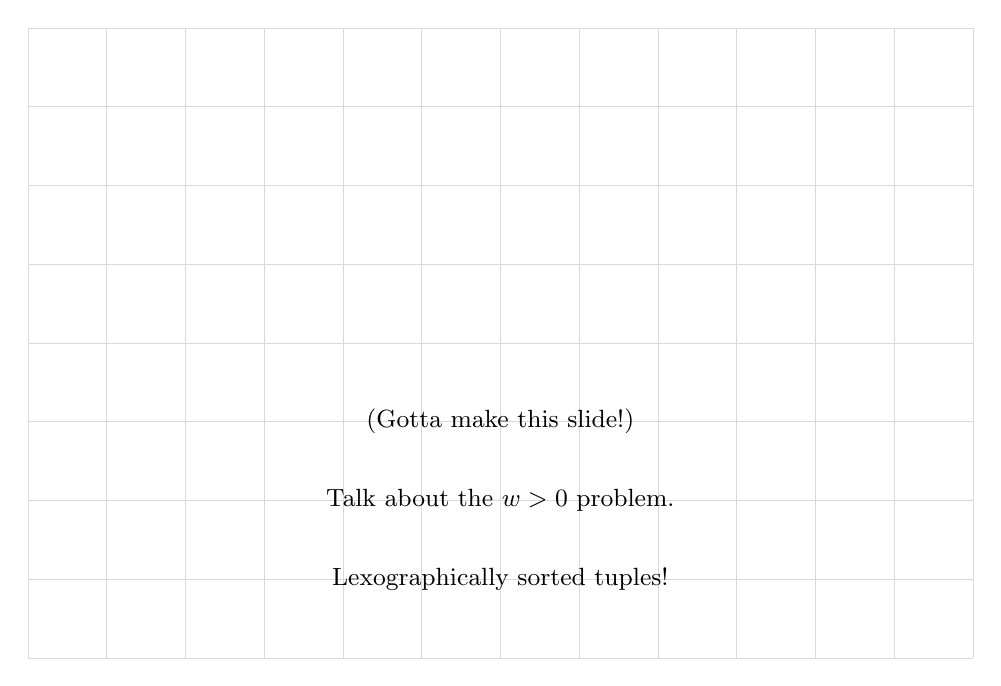
\begin{tikzpicture}[font=\small]
      \tikzset{>=latex} % arrow heads
      \draw[step=1,black!15,very thin,opacity=\gridopacity] (0,0) grid (12,8);

   \node at (6,3) {(Gotta make this slide!)};

   \node at (6,2) {Talk about the $w > 0$ problem.};
   \node at (6,1) {Lexographically sorted tuples!};

   \end{tikzpicture}
\end{frame}

\begin{frame}
   \frametitle{Traffic Problem Results: With Euclidean Heuristic}
   \begin{tikzpicture}[font=\small]
      \tikzset{>=latex} % arrow heads
      \draw[step=1,black!15,very thin,opacity=\gridopacity] (0,0) grid (12,8);

      \node at (6,3.8) {\includegraphics{build/incbi-road-ne/stats2vert}};

   \end{tikzpicture}
\end{frame}

\begin{frame}
   \frametitle{Revisiting LazySP Problems}
   
\begin{tikzpicture}[font=\small]
      \tikzset{>=latex} % arrow heads
      \draw[step=1,black!15,very thin,opacity=\gridopacity] (0,0) grid (12,8);

   \end{tikzpicture}
\end{frame}

\begin{frame}
   \frametitle{Experiment: Traffic Problem (VIDEO)}

   \begin{center}
      INSERT VIDEO!
   \end{center}
   
\end{frame}


\begin{frame}
   \frametitle{Summary}

   Summary of this portion of the talk!

   IBiD is a generalization of
   bidirectional Dijkstra's (from Goldberg),
   heuristic bidirectional Dijkstra's (from Goldberg),
   which each search from DynamicSWSF-FP.

   ... in the same way that LPA* is a generalization of A*
   and DynamicSWSF-FP (RR96).

   Experiments on LazySP problems later in the talk.
\end{frame}
